\documentclass[11pt,twoside]{book}

\usepackage{template/capaCinco}

\title{Coffee App}
\subtitle{E01-Definición del Proyecto}
\proyecto{Desarrollo de una aplicación móvil para mejorar el tiempo de respuesta de pedidos de una cafetería}
\productOwner{el de la café}
\equipo{Lolicon Team}{Francisco Isidoro Mera Torres}{Cedillo Vázquez Eliot Uriel}{Martinez Calderón Fernando}{Mejía Mendoza Diana Laura}{Eric Alejandro López Ayala}
\date{}

\begin{document}
	\LRCornerWallPaper{0.1}{template/img/izq}
	\maketitle
	\LRCornerWallPaper{0.1}{template/img/izq}
	\tableofcontents
	\listoffigures
	
	\newpage
	\projectCharter
	\firmas
	
	\chapter{Introducción}
	%!TEX root = ../prueba.tex
El presente documento tiene como propósito presentar la etapa de análisis y diseño del módulo de Autenticación y de Usuarios para el proyecto que se llevará a cabo durante el periodo escolar 2018-2019/1 en la Escuela Superior de Cómputo para la unidad de aprendizaje \textit{Desarrollo de Aplicaciones para Dispositivos Móviles}.Este proyecto está planeado y diseñado como lo indica el marco de trabajo Scrum y con un enfoque que se basa en los principios definidos en el \href{http://agilemanifesto.org}{Manifesto para el Desarrollo de Software ágil}.

\section{Estructura del documento}

En esta sección se describen brevemente los capítulos que conforman este documento así como notas, observaciones o comentarios adicionales que tienen como propósito apoyar en su lectura. El documento está estructurado de la siguiente forma:

\begin{itemize}
	\item En el capítulo \ref{ch:glosario} se enlistan los conceptos más relevantes del negocio sobre los cuales se

	\item Parte Uno: 
		La parte uno del documento está orientada a definir aquellos aspectos del sistema que no describen su comportamiento utilizando la especificación \textit{UML}.
		\begin{itemize}
			\item En el capítulo \ref{ch:arq} se utilizan diagramas para definir la arquitectura lógica del sistema. Esta definición a grandes rasgos identifica a los actores y la interacción directa de estos con el sistema, en en el capítulo \ref{ch:casosDeUso} se detalla esta interacción a través de historias de usuario.
		
			\item En el capítulo \ref{ch:modeloDeInformacion} se utiliza un diagrama de clases y tablas para mostrar la relación que existe entre las definiciones, términos y entidades relevantes en el negocio que permiten modelar su interacción con los actores del sistema. 		
				
			\item En el capítulo \ref{ch:reglas} se realiza la descripción de las normas, leyes o estrategias más relevantes que se deben aplicar al módulo, y en general considerarse en el proyecto para su implementación. 
			
		\end{itemize}
	\item Parte Dos: \hspace{1pt}
	Modelo Dinámico.
		\begin{itemize}
			\item En el capítulo \ref{ch:maquinas} se realiza la descripción de los estados o condiciones de   entidades o términos del negocio durante los procesos que en este documento se describen en el capítulo \ref{ch:casosDeUso}
			\item En el capítulo \ref{ch:casosDeUso} se realiza la descripción de los requerimientos que se presentaron en el documento \textit{E01-Especificación del Proyecto} utilizando casos de uso como método de especificación.
		\end{itemize}
	\item Parte Tres: Diseño
		\begin{itemize}
			\item En el capítulo \ref{ch:interfaces} se describen las interfaces que serán utilizadas por el Cliente en la aplicación móvil.
			\item En el capítulo \ref{ch:bd} se describe la notación y nomenclatura de la base de datos del sistema.
			\item En el capítulo \ref{ch:arquitectura} se describe la arquitectura física del sistema así como la arquitectura lógica de la aplicación móvil y la aplicación web.
			\item En el capítulo \ref{ch:mensajes} se describen los mensajes que el sistema utilizará para notificar a los actores cuando existen errores u operaciones exitosas.
		\end{itemize}	
\end{itemize}

\section{Notación y Nomenclatura}

Cada capítulo utiliza la siguiente nomenclatura para identificar a los diferentes elementos que conforman al documento.

\begin{Citemize}
	\item Para identificar a los stakeholders se utiliza el prefijo \textit{ST}.
	\item Para identificar a los requerimientos funcionales se utiliza el prefijo \textit{REQMXXYY} donde $xx$ es una abreviatura para el módulo al que pertenece el requerimiento y  $yy$ es un dígito del $0$ al $99$ que sirve como identificador único para el requerimiento.
	\item Para identificar a los requerimientos no funcionales se utiliza el prefijo \textit{REQNFXX} donde $xx$ es un dígito único del $0$ al $99$.
	\item Para identificar los entregables se utiliza el siguiente esquema:EXX-CYY-SPZZZ donde XX puede ser:
			\begin{Citemize}
				\item 02 - Análisis y Diseño.
				\item 03 - Implementación.
				\item 04 - Manual de Usuario.
			\end{Citemize}
		 YY puede ser:
		 	\begin{Citemize}
				\item 01 - Módulo de Autenticación.
				\item 02 - Módulo del Proveedor del Servicio.
				\item 03 - Módulo del Cliente.
				\item 04 - Módulo de Pagos.
			\end{Citemize}
		Y ZZZ es un dígito del 0 al 999 para especificar el Sprint en el cual se está trabajando. Si el entregable no tiene las letras SPZZZ entonces se trata de la recopilación de todos los sprints.
\end{Citemize}


	
	\chapter{Problemática}
	\label{ch:bc}
	%!TEX root = ../prueba.tex

\section{Contexto}

En Zacatenco, como en la mayoría de zonas escolares en la Ciudad de México, existe una cantidad considerable de proveedores de servicios de alimentos y bebidas, los cuales a veces tienen un espacio dentro de las instalaciones de las escuelas y otras veces se ubican fuera de las mismas. Estos establecimientos se enfrentan día a día a grandes olas de clientes que los prefieren por sabor, ambiente o cercanía con el único fin de alimentarse durante su tiempo libre o tiempo de receso. Muchas veces, el personal de estos establecimientos no se da abasto en recursos y tiempo para atender a la mayoría de los clientes que los visitan.

\subsection{Identificación del Problema}

El problema que identificamos tras una lluvia de ideas fue el siguiente:\\

\begin{center}\textit{El tiempo que un cliente debe esperar para ser atendido y recibir su comida o botana en un servicio de cafetería sobrepasa su tiempo libre o de receso.}\end{center}

Encontramos las siguientes causas más comunes del problema que mencionamos anteriormente son las siguientes:
	\begin{itemize}
		\item Pocas personas atendiendo la caja o preparando la comida.
		\item Un control de recursos(alimentos) que no responde a la demanda a tiempo.
	\end{itemize}

Tras una breve encuesta a la comunidad de la Escuela Superior de Cómputo, encontramos las siguientes consecuencias del problema que mencionamos anteriormente:
	\begin{itemize}
		\item Un cliente siente enojo cuando no obtiene el producto que deseaba o quería en el momento en el que se formó.
		\item Un cliente se siente estresado al esperar en una fila muy larga.
		\item Un cliente le da preferencia a la competencia al tener menos personas esperando por sus pedidos.
	\end{itemize}
	
	
\subsection{Identificación de Stakeholders/Actores del Sistema}

Los stakeholders son aquellas personas que se verán afectadas de forma directa o indirecta por la realización y conclusión del proyecto. A lo largo de está sección se presentan a los roles que se han identificado y que van a interactuar de forma directa con el sistema utilizando la aplicación móvil o la aplicación web. Para representar a los stakeholders, se utiliza la especificación \textit{UML} para actores.\\

En la figura \ref{fig:organigrama} se muestra la estructura jerárquica y generalizada de una cafetería, esto con el fin de identificar, separar y priorizar los requerimientos de los actores del sistema y hacer la estimación correspondiente de tiempo y costos. El organigrama también nos permite definir parte del diagrama de actores del sistema bajo el cual se harán las relaciones correspondientes con las user stories que se pueden observar al finalizar el siguiente capítulo.

\begin{figure}[hbtp!]
	\begin{center}
		\fbox{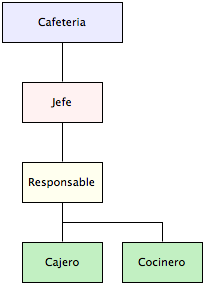
\includegraphics[width=0.3\textwidth]{img/organigrama}}
		\caption{Organigrama de una Cafetería}
		\label{fig:organigrama}
	\end{center}
\end{figure}


En la figura \ref{fig:actores} se muestra un diagrama en \textit{UML} que tiene como propósito representar cómo está dividido el sistema en función de los stakeholders identificados. A continuación se enlistan las observaciones más relevantes de este diagrama.
\begin{Citemize}
	\item La \getElementById[Stakeholder]{Persona} es un actor abstracto el cual tiene como principal objeto generalizar las funcionalidades a las que todos los actores del sistema tendrán acceso independientemente de su rol como por ejemplo iniciar sesión o recuperar su cuenta.
\end{Citemize}

\begin{figure}[hbtp!]
	\begin{center}
		\fbox{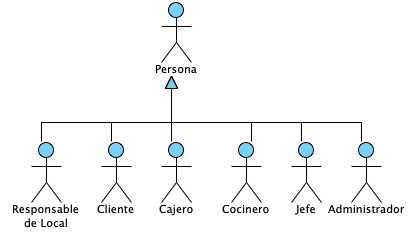
\includegraphics[width=0.5\textwidth]{img/actores}}
		\caption{Actores del Sistema}
		\label{fig:actores}
	\end{center}
\end{figure}

A continuación se hará la descripción formal de cada uno de los actores(ó stakeholders) del sistema. Esta descripción incluye un breve resumen del actor, sus responsabilidades en el sistema y el perfil que una persona debe cubrir para tener este rol.


\begin{Actor}{Persona}{Persona}{Un usuario es toda persona que va a interactuar con el sistema mediante la aplicación móvil o la aplicación web.}
	\item[Responsabilidades:] No aplica.
	\item[Perfil]:\hspace{1pt}
		\begin{itemize}
			\item Alumno de nivel medio superior, superior o posgrado del I.P.N. o de U.N.A.M.
			\item Docente de nivel medio superior, superior o posgrado del I.P.N. o de U.N.A.M.
			\item Personal externo en una unidad académica del I.P.N. o escuela de la U.N.A.M.
			\item Personal de una cafetería.
		\end{itemize}
\end{Actor}

\begin{Actor}{Jefe}{Jefe}{También conocido como \textbf{Dueño} es la persona que legalmente tiene derecho a utilizar el nombre de una franquicia para abrir uno o más locales en determinados espacios, dentro o fuera de una unidad académica del I.P.N. así como una escuela de otra Institución Educativa.}
	\item[Responsabilidades:] \hspace{1pt}
		\begin{itemize}
			\item Agregar al sistema a los empleados.
			\item Designar un responsable del local.
			\item Tomar desiciones ejecutivas que respondan a las demandas de su establecimiento con base en 			gráficas o datos estadísticos.
			\item Definir las horas de operación de un local.
		\end{itemize}
	\item[Perfil]:\hspace{1pt}
		\begin{itemize}
			\item Licenciatura.
			\item Responsable.
			\item Líder.
		\end{itemize}
\end{Actor}


\begin{Actor}{Administrador}{Administrador}{Es la persona que se encargará de desbloquear cuentas de usuario en el sistema así como de vigilar y mejorar las respuestas del sistema una vez sea puesto en producción.}
	\item[Responsabilidades:]\hspace{1pt}
		\begin{itemize}
			\item Desbloquear cuentas de usuario que estén bloqueadas.
		\end{itemize}
	\item[Perfil:]\hspace{1pt}
		\begin{itemize}
			\item Licenciatura en Computación, Ingeniería en Sistemas Computacionales o a fin concluida.
			\item Conocimientos Avanzados en Tunning y Performance de bases de datos.
		\end{itemize}
\end{Actor}


\begin{Actor}{ResponsableDeLocal}{Responsable de Local}{Es la persona encargada de administrar la información de una cafetería como lo es el nombre de la cafetería, ubicación, escuelas a las que generalmente atiende y los productos en inventario.}
	
	\item[Responsabilidades:]\hspace{1pt}
		\begin{itemize}
			\item Vigilar que los reglamentos internos y de salubridad se cumplan y hacer cumplir las sanciones correspondientes.
			\item Administrar la información de los productos que se venden en su local.
			\item Vigilar que el proceso de surtido se lleve a cabo de forma correcta.
		\end{itemize}
	
	\item[Perfil:]\hspace{1pt}
		\begin{itemize}
			\item Experiencia en administración de empresas.
			\item Responsable.
			\item Honesto.
		\end{itemize}
	
\end{Actor}
		
\begin{Actor}{Cocinero}{Cocinero}{Es una persona que pertenece a una o más cafeterías y que tiene como principal responsabilidad atender pedidos y cocinarlos o delegarle esta responsabilidad a otro cocinero dentro de la misma cafetería.}
	
	\item[Responsabilidades:] \hspace{0.5cm}
		\begin{itemize}
			\item Monitoreo, control y conservación de los insumos de la cocina.
			
			\item Colaborar en la planificación de menús.
			
			\item Ayudar a administrar los costos e inventario.
			
			\item Dividir, conducir y organizar el trabajo con otros miembros del staff en la preparación de las ordenes.
			
			\item Iteractuar con el proveedor del servicio.
			
			\item Atender y preparar los pedidos solicitados por los clientes.
		\end{itemize}
	
	\item[Perfil:] \hspace{0.5cm}
		\begin{itemize}
			\item Excelentes habilidades de comunicación.
			
			\item Buenos estándares de higiene.
			
			\item Organizado y metódico.
			
			\item Experiencia en cáterin.
		\end{itemize}
	
	\end{Actor}
	
	
	\begin{Actor}{Cajero}{Cajero}{Es una persona que pertenece a una o más cafeterías y que tiene como propósito cobrar los pedidos de los clientes.}
	
	\item[Responsabilidades:] \hspace{0.5cm}
		\begin{itemize}
			\item Recibir dinero en efectivo, de requerirlo realiza arqueos de caja.
			
			\item Es el responsable directo de dinero en efectivo.
			
			\item Registrar operando una caja los movimientos de entrada y salida de dinero.
			
			\item Informar a su superior los movimientos diarios de la caja.
			
			\item Mantener en orden el equipo y sitio de trabajo, reportando cualquier anomalia.
			
			\item Manejar un grado de confidencialidad sobre las transacciones bajo.
		\end{itemize}
	
	\item[Perfil:] \hspace{0.5cm}
		\begin{itemize}
			\item Excelentes habilidades de comunicación , para atención al cliente.
			
			\item Habilidades numericas.
			
			\item Actitud de servicio.
			
			\item Proactivo.
			
			\item Responsable.
			
			\item Buena gestión de tiempo.
		\end{itemize}
	
	\end{Actor}

	\begin{Actor}{Cliente}{Cliente}{Es cualquier persona(alumno, profesor, personal externo) que consume o adquiere los productos de una cafetería para consumirlos.}
	
	\item[Responsabilidades:]\hspace{1pt}
		\begin{itemize}
		\item Confirmar los pedidos que se realicen en el sistema.
		\item Realizar el pago correspondiente por los productos solicitados y consumidos.
		\end{itemize}
	\item[Perfil:]\hspace{1pt}
		\begin{itemize}
			\item Alumno de nivel medio superior, superior o posgrado del I.P.N. o de U.N.A.M.
			\item Docente de nivel medio superior, superior o posgrado del I.P.N. o de U.N.A.M.
			\item Personal externo en una unidad académica del I.P.N. o escuela de la U.N.A.M.
		\end{itemize}
	\end{Actor}
	
	
	\chapter{Propuesta de Solución}
	\label{ch:ps} 
	%!TEX root = ../prueba.tex
\section{Introducción}

En el capítulo anterior se identificó un problema, se enlistaron sus causas y consecuencias. En este capítulo se describirá lo que el equipo propone para resolver este problema utilizando diagramas bajo la especificación de \textit{UML} del \textit{Business Process Modeling} y la visión del proyecto, la cual se presenta a continuación.\\

{\em{Diseñar e implementar un sistema que mejore el tiempo de respuesta de una cafetería para atender pedidos a clientes en horas de alta concurrencia.\\}}

\section{Descripción de la Propuesta}
El diagrama que se muestra en la figura \ref{fig:bpmn} muestra las actividades o tareas que deberá realizar cada actor del sistema para que se cumpla con la visión del proyecto. A continuación se enlistan estas tareas y se hace una descripción breve de qué consisten, cabe mencionar que el flujo de este diagrama es el ideal. También es pertinente hacer la observación de que este flujo es para aquellos pedidos que requieren ser atendidos por la cocina del local y que ya han sido pagados por una de las formas de pago disponibles. Si el contenido del pedido es únicamente de abarrotes no es requerido notificar a la cocina y sólo se procede a realizar el pago de forma habitual.

\begin{figure}[hbtp!]
	\begin{center}
		\fbox{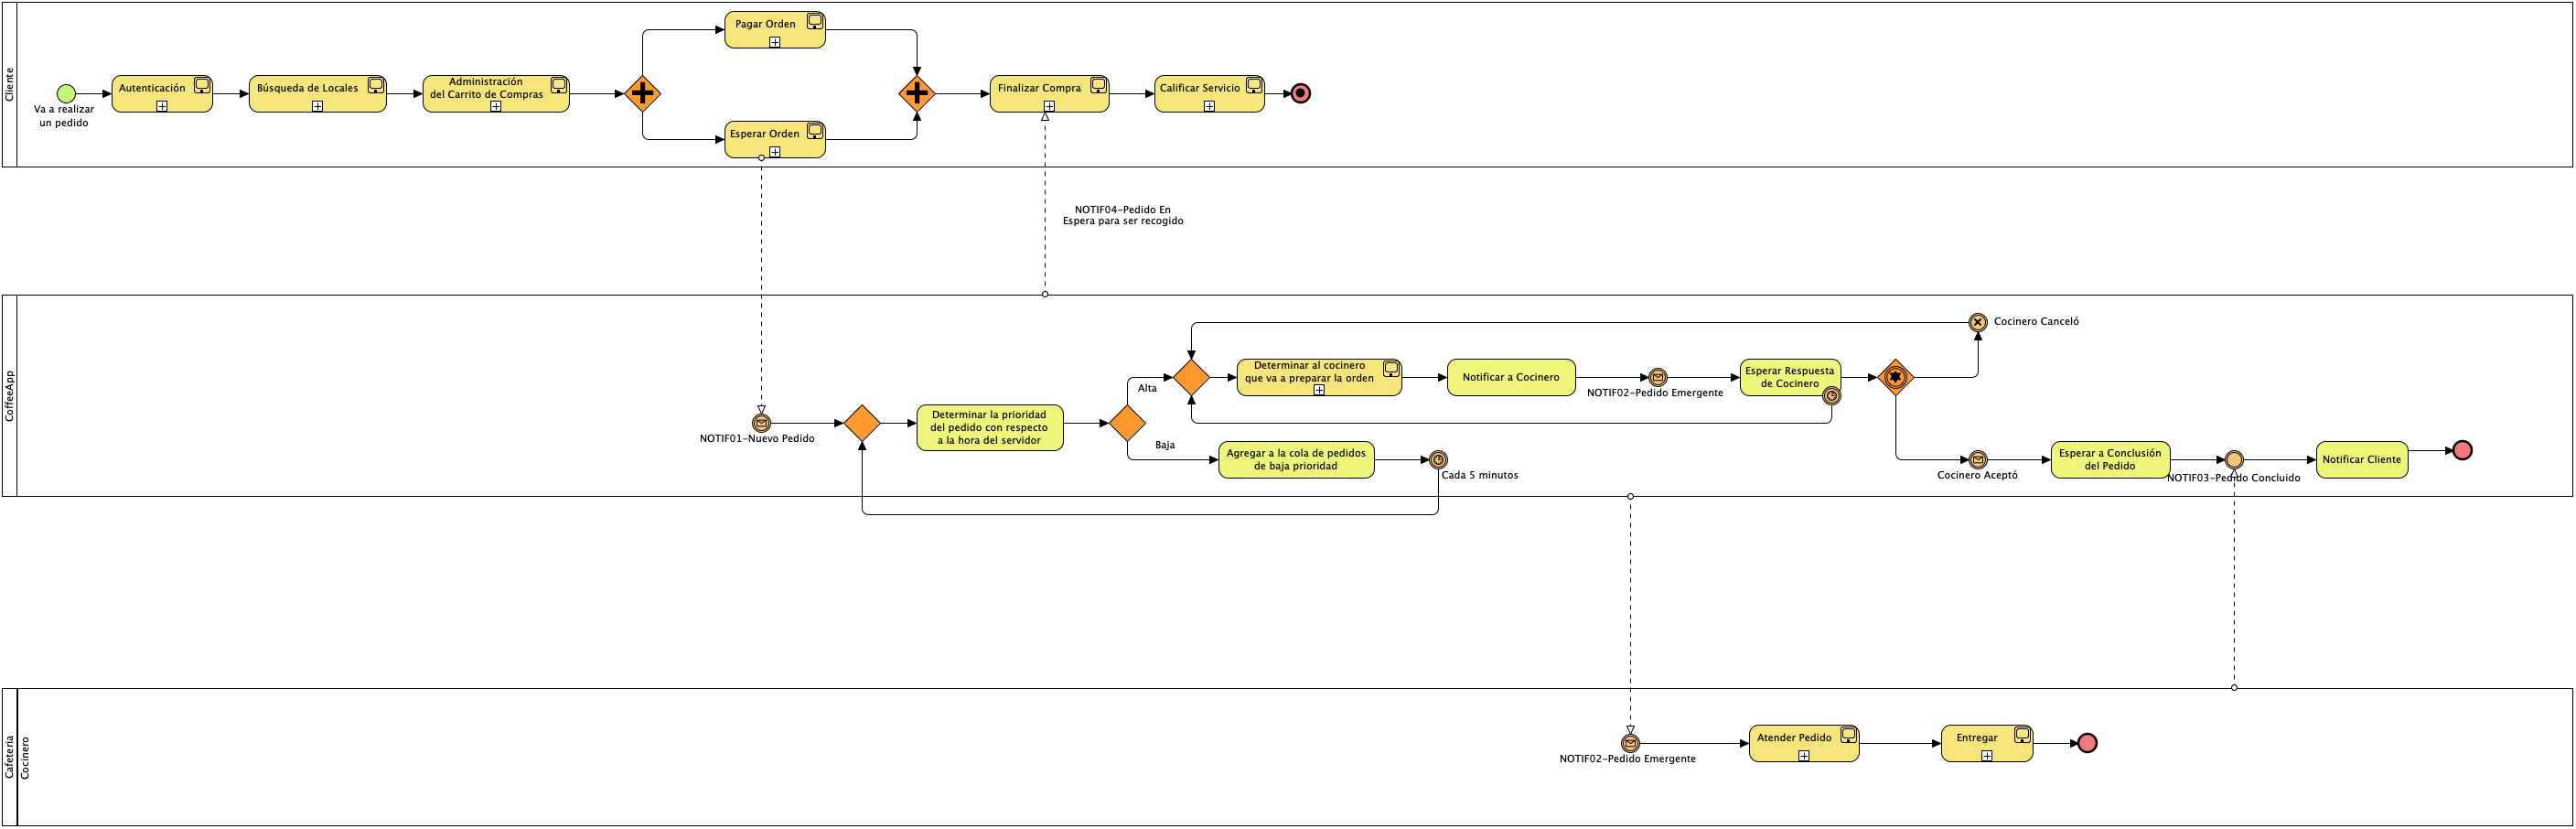
\includegraphics[width=\textheight,angle=90]{img/PropuestaDeSolucion}}
		\caption{Propuesta de Solución}
		\label{fig:bpmn}
	\end{center}
\end{figure}

\begin{description}
	\item[Cliente:]\hspace{1pt}
		
		\begin{enumerate}
			\item \label{PROC01Cliente:inicio} \init El proceso inicia cuando el cliente va a utilizar la aplicación móvil. Continúa el sub proceso de autenticación en el paso \ref{PROC01Cliente:autenticacion}.
			\item \label{PROC01Cliente:autenticacion}\process En el proceso de autenticación el cliente iniciará sesión en la aplicación móvil o en su defecto se registrará. Continúa con el paso \ref{PROC01Cliente:consultarLocales}
			\item \label{PROC01Cliente:consultarLocales}\task El dispositivo móvil desde el cual el cliente inicia sesión le proporciona a la aplicación móvil una ubicación geográfica aproximada, la aplicación móvil le desplegará en pantalla al cliente los locales más cercanos a su posición en un radio aproximado de 2 kilómetros. Continúa con el paso \ref{PROC01Cliente:seleccionarLocal}.
	\item \label{PROC01Cliente:seleccionarLocal} \task El cliente selecciona un local de su preferencia ya sea de los desplegados en el paso \ref{PROC01Cliente:consultarLocales} o utilizando la aplicación para buscar un local en particular. Continúa con el paso \ref{PROC01Cliente:consultarListaDeProductos}.
			\item \label{PROC01Cliente:consultarListaDeProductos}\task El cliente indica que va a comprar uno o más productos consulta la lista de productos disponibles del local seleccionado en el paso \ref{PROC01Cliente:seleccionarLocal}. Continúa con el paso \ref{PROC01Cliente:administrarCarritoDeCompras}.
			\item \label{PROC01Cliente:administrarCarritoDeCompras}\process El cliente seleccionará los productos que va a comprar en la aplicación móvil. Continúa con el paso \ref{PROC01Cliente:indicarTipo}. En este proceso se especificará el método de pago así como la posibilidad de agregar notas adicionales a los productos solicitados que así el cliente lo requiera.
			\item \label{PROC01Cliente:indicarTipo} \task El cliente indicará en la aplicación si su pedido debe ser enviado de forma inmediata a la cocina o se debe enviar en una hora en particular.
			\item \label{PROC01Cliente:gateUno} \gate Si el pedido del cliente es del tipo inmediato se continúa con el paso \ref{PROC01Cliente: confirmarPedido}, en caso de que el pedido del cliente sea de tipo programado se continúa con el paso \ref{PROC01Cliente:indicarHora}. 
			\item \label{PROC01Cliente:indicarHora} \task El cliente indicará la hora en la que quiere que su pedido llegue a la cocina para ser atendido por algún cocinero. Continúa con el paso \ref{PROC01Cliente:confirmarPedido}.
			\item \label{PROC01Cliente:confirmarPedido} \task El cliente indicará a la aplicación que va a ir al local seleccionado para recoger su pedido. 
			\item \label{PROC01Cliente:notif} Cuando el pedido del cliente ha sido preparado y empaquetado para su recepción el cliente irá al local seleccionado y recogerá su pedido y concluye el flujo.
		\end{enumerate}
	
	\item[Coffee App:]\hspace{1pt}
		\begin{enumerate}
			\item \label{PROC01App:ValidarExistencia}\task La aplicación móvil deberá validar la existencia de los productos contenidos en el carrito de compras en el local que el cliente haya seleccionado para realizar su pedido.
			\item \label{PROC01App:notif} La aplicación recibe y atiende la notificación de un nuevo pedido ejercida por un cliente y continúa con el paso \ref{PROC01App:servidor}.	
			\item \label{PROC01App:servidor} \task Si la prioridad de el pedido es alta, es decir el tipo del pedido es inmediato se debe continuar con el paso \ref{PROC01App:notificarCocina}. En caso contrario, el pedido es de tipo programadom, por lo que el pedido pasará a formar parte de una estructura de datos que será revisada por otro proceso, el cual determinará si el pedido debe ser notificado a la cocina o continuar en espera.
			\item \label{PROC01App:notificarCocina} \task Cuando la prioridad de un pedido es alta se mandará una notificación a los cocineros que estén disponibles en local para ser atendida.
			\item \label{PROC01App:atencionPedido} Cuando un cocinero ha seleccionado atender un pedido la aplicación recibe la notificación correspondiente y continúa con el paso \ref{PROC01App:horaDeAtencion}.
			\item \label{PROC01App:horaDeAtencion} \task La aplicación móvil calculará la hora aproximada en la que el cocinero atenderá el pedido con base en sus pedidos anteriores. Continúa con el paso \ref{PROC01App:calcularHoraFinalizacion}.
			\item \label{PROC01App:calcularHoraFinalizacion} \task La aplicación móvil calculará la hora aproximada en la que el cocinero concluirá la preparación del pedido. Continúa con el paso \ref{PROC01App:notificarCliente}.
			\item \label{PROC01App:notificarCliente} \task La aplicación móvil le notificará al cliente la hora aproximada en la que podrá ir al local a recoger su pedido.
			\item \label{PROC01App:pedidoNoEntregado} Cuando un pedido no ha sido recogido en el lapso de 15 minutos la aplicación mandará una notificación a los clientes que hayan realizado al menos una compra en ese local para recoger y realizar el pago correspondiente por el pedido.
		\end{enumerate}

	\item[Cocinero:]\hspace{1pt}
		\begin{enumerate}
			\item \label{PROC01Cocinero:notif} Una vez que se ha determinado que un pedido tiene prioridad alta se notificará a la cocina para que un cocinero atienda el pedido. Continúa con el paso \ref{PROC01Cocinero:seleccionarPedido}.
			\item \label{PROC01Cocinero:seleccionarPedido} \task El cocinero selecciona el pedido emergente para indicar que lo va a atender. Cuando un pedido emergente no ha sido seleccionado por algún cocinero, se le notificará al cliente que hay un retraso aproximado de 5 minutos para atender su orden, más sin en cambio un cocinero indica que vas a atender un pedido el sistema realizará los cálculos correspondientes para determinar el tiempo estimado de entrega. Continúa con el paso \ref{PROC01Cocinero:atender}.
			\item \label{PROC01Cocinero:atender} \task El cocinero atiende el pedido preparándolo. Continúa con el paso \ref{PROC01Cocinero:espera}.
			\item \label{PROC01Cocinero:espera} \task Una vez el cocinero indicó que ha concluido de preparar el pedido del cliente, la aplicación comenzará a tomar el tiempo para que el cliente pase al local correspondiente a recoger su pedido. Si el cliente llegó en un lapso menor a 15 minutos se continúa con el paso \ref{PROC01Cocinero:entrega},en caso contrario se continúa con el paso \ref{PROC01Cocinero:oferta}.
			\item  \label{PROC01Cocinero:entrega} \task Cuando el cliente llegó en el rango de tiempo de 0 a 15 minutos se le hará entrega de su pedido y finaliza el proceso.
			\item \label{PROC01Cocinero:oferta} \task Cuando el cliente no llegó en el rango de tiempo de 0 a 15 minutos el cocinero indicará que el pedido puede ser tomado por otro cliente que pague por él en un tiempo limitado de 15 minutos. Continúa con el paso \ref{PROC01Cocinero:entrega}.
		\end{enumerate}

\end{description}


\section{Arquitectura Física}

En esta sección se realizar la especificación técnica y física de la arquitectura sobre la cual la aplicación y el sistema funcionaran desde su puesta en producción. Dicha especificación se realiza utilizando como base la figura \ref{fig:arqFisica}.

\begin{figure}[hbtp!]
	\begin{center}
		\fbox{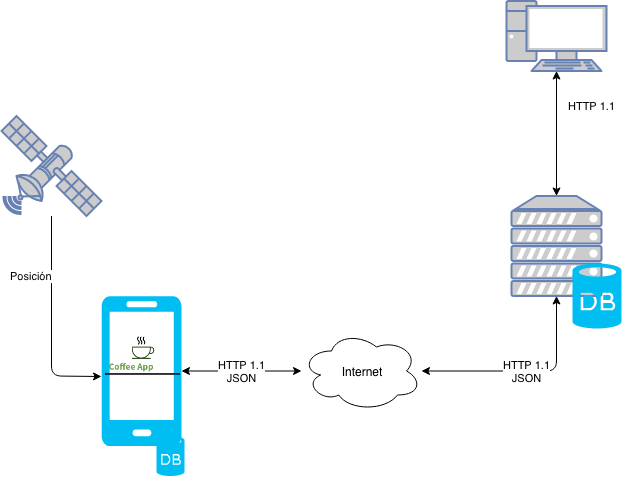
\includegraphics[width=.5\textwidth]{img/arqFisica}}
		\caption{Arquitectura Física del Sistema}
		\label{fig:arqFisica}
	\end{center}
\end{figure}

\subsection{Arquitectura Base}
El sistema está pensado para trabajar bajo un esquema centralizado tomando como base la arquitectura \textbf{Cliente-Servidor}. Esta arquitectura nos sirve como punto de partida debido a dos principales razones:
	\begin{itemize}
		\item Es requerido un punto centralizado(servidor) donde se almacene la mayor cantidad de información y que sea un punto de acceso para varios dispositivos.
		\item Es requerido hacer la implementación de dos diferentes clientes desde los cuales se tendrá acceso al servidor y por consiguiente a la información. El primer cliente consta de una aplicación móvil para dispositivos con sistema operativo Android, el segundo cliente consta de una aplicación web basada en \textit{Servlets} y \textit{JSP's}. 
	\end{itemize}

Se optó también por utilizar como base la arquitectura \textbf{Cliente - Servidor} ya que nos permite el uso del protocolo \textit{HTTP 1.1} para crear varios canales de comunicación entre los distintos clientes que accederán al sistema. El protocolo \textit{HTTP} nos define que para que exista comunicación entre el Cliente y el Servidor se debe hacer uso de dos mecanismos: una \textit{Petición} y una \textit{Respuesta}. A grandes rasgos, la petición está formada entre otras cosas por cabeceras, métodos y parámetros los cuales son enviados desde el cliente a través de la red hasta llegar al servidor el cual debe validar que la \textit{URL} desde la cual se hace la petición es válida. Posteriormente el servidor procesa la petición y en caso de existir el recurso y el método contenido en la petición le devolverá al cliente una respuesta con la información solicitada utilizando el formato indicado en el \textit{MIME/TYPE} de la respuesta.\\

Los actores que podrán acceder al sistema mediante la aplicación web son:
	\begin{itemize}
		\item El \getElementById[Stakeholder]{Jefe} dado que es el encargado de registrar, editar o eliminar la información de las cafeterías de las que es dueño así como sus respectivos locales y productos que se podrán encontrar en todos los locales de su franquicia.
		\item El \getElementById[Stakeholder]{Administrador} dado que es el encargado de habilitar el acceso a las personas que tienen una cuenta bloqueada al sistema.
		\item El \getElementById[Stakeholder]{ResponsableDeLocal} dado que es el encargado de registrar la información de los productos que se ofertan en un local.
	\end{itemize}

Los actores que tendrán acceso a la aplicación móvil son:
	\begin{itemize}
		\item El \getElementById[Stakeholder]{Cliente} dado que desde su dispositivo únicamente podrá consultar información de las cafeterias, locales y productos publicados para realizar pedidos que serán atendidos por el personas de los locales, la aplicación móvil hará uso de dos mecanismos relevantes:
		\begin{itemize}
			\item El módulo GPS ya que cuando el cliente acceda a la aplicación se determinará su posición y con esto la ubicación de los locales más cercanos en un radio de 2 kilómetros.
			\item Una base de datos local que almacenará los pedidos que no han sido confirmados para que el cocinero de un local inicie su preparación.
		\end{itemize}
		\item El \getElementById[Stakeholder]{Cocinero} dado que a su tableta o a la tableta proporcionada por la cafetería, atenderá los pedidos e indicará la conclusión de su preparación para que se le entrege al cliente.
\end{itemize}


\subsection{Especificaciones Técnicas}
A continuación se especifican los detalles técnicos del sistema, es decir, el Hardware y Software requerido para que el sistema opere de forma estable.

\subsubsection{Servidor}
El servidor tiene las siguientes especificaciones:
	\begin{description}
		\item[Marca:]Servidor Dell PowerEdge T30.
		\item[Procesador:]Intel Xeon E3-1225V5 3.30GHz.
		\item[Memoria RAM:]8GB DDR4.
		\item[Disco Duro:]1TB.
		\item[Sistema Operativo:] CentOS 7.4-1708.
	\end{description}

\subsection{Base de Datos}
	\begin{description}
		\item[SGBD:] Postgresql 9.4
	\end{description}

\subsubsection{Cliente Web}
La aplicación web puede ser utilizada bajo las siguientes especificaciones:
	\begin{description}
		\item[Navegadores Compatibles:]\hspace{0.5pt}
			\begin{itemize}
				\item Google Chrome Versión $\geq$ 70.0.3538.
				\item Mozilla Firefox $\geq$ 63.0.
				\item Safari $\geq$ 12.0.
			\end{itemize}
		\item[Resolución:]\hspace{0.5pt}
			\begin{itemize}
				\item Mínima:1027x768
				\item Máxima:1920x1080
			\end{itemize}
	\end{description}

\subsubsection{Cliente Móvil}
La aplicación móvil puede ser utilizada bajo las siguientes especificaciones:
	\begin{description}
		\item[Sistema Operativo:] Android >= 5.0 Lollipop.
		\item[Memoria RAM:] 2GB.
		\item[Almacenamiento:] 16 GB.
	\end{description}


\section{Arquitectura Lógica}
Una vez descrita la arquitectura física del sistema, es requerido indicar y especificar cómo será construido. En general las aplicaciones que se van a desarrollar utilizarán una arquitectura a capas. En la figura \ref{fig:arqLogica} se pueden observar las capas del sistema en los diferentes clientes(o aplicaciones) y posteriormente se hará una descripción de la función de cada capa.

\begin{figure}[hbtp!]
	\begin{center}
		\fbox{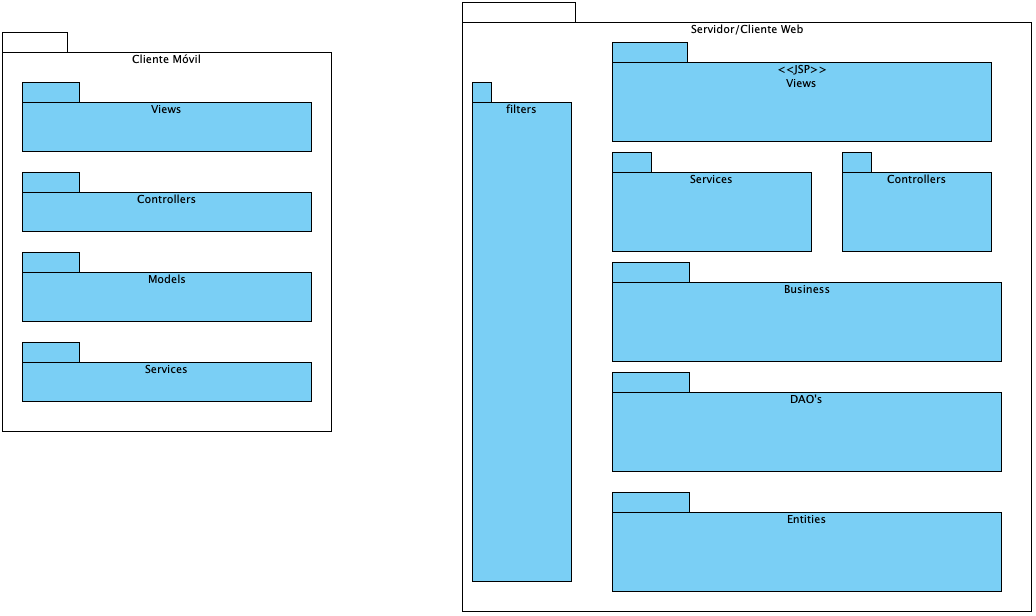
\includegraphics[width=0.8\textwidth]{img/arqLogicaP}}
		\caption{Arquitectura Lógica del Sistema}
		\label{fig:arqLogica}
	\end{center}
\end{figure}

\subsection{Arquitectura Lógica del Servidor/Aplicación Web}
Como se mencionó al iniciar esta sección, las aplicaciones están construidas a partir de una arquitectura multi capa.El servidor(paquete del lado derecho en la figura \ref{fig:arqLogica}) está dividido en las siguientes capas:
	\begin{description}
		\item[Entities:] En esta capa se definen las clases que se utilizarán para la manipulación de las estructuras de datos de la base de datos.
		\item[DAO's:] En esta capa se definen las clases que sirven de interacción entre la capa de \textit{business} y la capa de \textit{entities} para la recolección de datos utilizando el patrón de diseño DAO.
		\item[Business:] En esta capa se definen las clases que sirven para la abstracción de las reglas de negocio así como de las operaciones y funciones disponibles en el sistema.
		\item[Services:] En esta capa se definen las clases que corresponden al servicio RESTful que será consumido por la aplicación móvil.
		\item[Controllers:] Está capa tiene el propósito establecido para la capa de \textit{Controlador} en el patrón de diseño \textit{MVC} en donde se va a administrar el flujo de datos que hay entre la capa \textit{views} y la capa \textit{business}.
		\item[Views:] Está capa contiene los archivos JPA's que presentan las interfaces de usuario para la aplicación web.
	\end{description}
	
\subsection{Arquitectura Lógica de la Aplicación Móvil}
La aplicación móvil se va a construir con base en el patrón arquitectónico \textit{MVC}, agregando una capa la cual tiene como principal propósito administrar las peticiones que se van a mandar al servidor y proveer de datos a la capa de \textit{Models}. Así mismo dado que la aplicación móvil es nativa del sistema operativo Android, se hará uso de algunos patrones de diseño establecidos por \textit{Google} para el comportamiento de algunos componentes como lo es el patrón \textit{Adapter} para el componente \textit{Recycler View}.





	
	\chapter{Alcance}
	\label{ch:al}
	%!TEX root = ../prueba.tex
En este capítulo se pueden encontrar los requerimientos iniciales del sistema que se identificaron durante la toma de requerimientos y de una lluvia de ideas.

\section{Requerimientos Funcionales}
%!TEX root = ../prueba.tex
\begin{ReqSpec}
	\Req{REQMU01}{Iniciar Sesión}{Autenticación}{Funcional}{Como usuario de la aplicación requiero de un mecanismo que me permita escribir mi correo electrónico o nombre de usuario y una contraseña, con el fin de autenticar mi persona y así realizar acciones dentro de la aplicación web o móvil que correspondan a mi perfil. Las acciones que puedo realizar en el sistema deben ser desplegadas en un menú.}{Alta}
	
	\Req{REQMU02}{Crear, modificar y eliminar cuenta de usuario}{Autenticación}{Funcional}{Como cliente y proveedor del sistema requiero de un mecanismo que permita ingresar mis datos personales: nombres y apellidos, teléfono móvil, correo electrónico, escuela o unidad académica, comida preferida, nombre de usuario y contraseña para así tener una forma de autenticarme y acceder a las funcionalidades de la aplicación de acuerdo a mi perfil. También requiero de un mecanismo que me permita modificar mis datos personales de la cuenta o eliminar mi cuenta en caso de ya no requerirla.}{Alta}
	
	\Req{REQMU03}{Recuperar Cuenta de Usuario}{Autenticación}{Funcional}{Como usuario de la aplicación requiero de un mecanismo que me permita recuperar mis datos de acceso al sistema en caso de extraviar u olvidar mi cuenta de usuario o contraseña envíandome un correo electrónico o mensaje SMS los datos actualizados.}{Alta}

	\Req{REQMU04}{Vincular cuenta de Google}{Autenticación}{Funcional}{Debe existir un mecanismo que como usuario me permita vincular una cuenta existente del proveedor de servicio Google con el fin de identificarme dentro de la aplicación y tener acceso a los servicios que correspondan segun el rol.}{Baja}
	
	\Req{REQMU05}{Vincular cuenta de Facebook}{Autenticación}{Funcional}{Debe existir un mecanismo que como usuario me permita vincular una cuenta existente del proveedor de servicio  Facebook con el fin de identificarme dentro de la aplicación y tener acceso a los servicios que correspondan segun el rol.}{Baja}
	\Req{REQMU06}{Iniciar Sesión con una cuenta temporal}{Autenticación}{Funcional}{Debe existir un mecanismo}{Baja}
\end{ReqSpec}
%!TEX root = ../prueba.tex
\begin{ReqSpec}
	\Req{REQMP01}{Agregar Nuevo Establecimiento, Editar Información de Establecimiento y Eliminar Establecimiento}{Proveedor de Servicio}{Funcional}{Como proveedor del servicio de cafetería requiero de un mecanismo que me permita agregar la información de mi establecimiento: nombre, descripción, ubicación geográfica, escuelas más cercanas y especialidades, también se requiere de un mecanismo que me permita actualizar o editar la información previamente mencionada o eliminar la información de mi establecimiento para que ya no aparezca en la lista de establecimientos.}{Alta}
	
	\Req{REQMP02}{Agregar Información de Proveedor, Editar Información de Proveedor y Eliminar proveedor}{Proveedor de Servicio}{Funcional}{Como proveedor de servicio requiero de un mecanismo que me permita tener un control de las empresas a las que se les pide generalmente productos, los datos que se deberán registrar de los proveedores son: nombre de la empresa, lista de productos que surte, teléfono de contacto y correo electrónico. Así mismo requiero de un mecanismo que me permita actualizar los datos previamente enunciados y de un mecanismo que me permita eliminar la información de un proveedor.}{Baja}
	
	\Req{REQMP03}{Agregar Producto a Inventario, Editar Información del Producto y Eliminar Producto de Inventario}{Proveedor de Servicio}{Funcional}{Como proveedor del servicio requiero de un mecanismo que me permita agregar la siguiente información de nuevos productos adquiridos:nombre, descripción, clasificación del producto, imagen, precio de venta, precio de adquisición. Así mismo, requiero de un mecanismo que me permita actualizar la información de un producto de mi inventario o eliminarlo en caso de haber un registro erróneo en la aplicación.}{Alta}
	
	\Req{REQMP04}{Registrar entrada de productos a la cafetería}{Proveedor de Servicio}{Funcional}{Como proveedor del servicio requiero de un mecanismo que me permita indicar cuando un pedido hecho a un proveedor llega a la cafetería para que esos productos pasen a formar parte de lo que se puede vender en el día. La información que requiero que se registre es: nombre de la persona que recibe, hora de entrada de los productos, la lista de productos y la cantidad de los productos en unidades, estado general del pedido y el estado particular de los productos.}{Alta}
	
	\Req{REQMP09}{Actualizar existencia de producto}{Proveedor de Servicio}{Funcional}{Como proveedor de servicio requiero de un mecanismo que por cada producto que sea vendido se actualice su existencia dentro de la cafetería con el fin de tener un control de los productos que todavía pueden ser vendidos.}{Alta}
		%Cambia el estado 
			%Stock > 10
			%A punto de agotarse 0 < p < 10
			%Agotado = 0
			
	\Req{REQMP05}{Agregar paquete, Editar Paquete y Eliminar Paquete}{Proveedor de Servicio}{Funcional}{Como proveedor de servicio requiero de un mecanismo que me permita armar paquetes para que los clientes compren de 3 a 5 productos con una reducción del costo configurable de entre 5\% y 10\% sobre el costo total de los productos que conforman el producto además de poder darle un nombre, descripción e imagen. También requiero de un mecanismo que me permita actualizar los productos que conforman un paquete, su precio, nombre, descripción e imagen.}{Alta}
	%Paquete 1:
		%Cafe
		%Torta
		%Gelatina
		
	\Req{REQMP06}{Consultar lista de pedidos}{Proveedor de Servicio}{Funcional}{Como proveedor de servicio requiero de un mecanismo que me permita consultar los pedidos de un establecimiento que están confirmados y en espera para seleccionar aquellos pedidos voy a cocinar o que estoy a punto de acabar para que el cliente pase por el.}{Alta}
	
	\Req{REQMP07}{Consultar pedido}{Proveedor de Servicio}{Funcional}{Como proveedor de servicio requiero de un mecanismo que me permita seleccionar un pedido y consultar las especificaciones del cliente.}{Alta}
	
	
	\Req{REQMP08}{Actualizar estado del pedido}{Proveedor de Servicio}{Funcional}{Como proveedor de servicio requiero de un mecanismo que:
		\begin{Citemize}
			\item Permita al cliente indicar que confirma su pedido, que cancela su pedido, que ha ido ha la caja y pagado su pedido.
			\item Me permita indicar que estoy preparando un pedido o que estoy a punto de terminar su preparación o me permita indicar cuando un pedido puede ser recogido por otro cliente cuando el que lo solicitó tardo más de 10 minutos en recogerlo.
		\end{Citemize}}{Alta}
		%Actualizar
			%Por confirmar
			%En espera
			%En preparación
			%A punto de terminar
			%Recogido y pagado
			%Cancelado
			%En espera de nuevo cliente
			
	\Req{REQMP10}{Reporte de la Experiencia del Cliente}{Proveedor de Servicio}{Funcional}{Como proveedor de servicio requiero de un mecanismo que me permita consultar la experiencia promedio de los clientes que visitan el establecimiento.}{Baja}
	
	\Req{REQMP11}{Agregar promoción, editar promoción, guardar promoción y eliminar promoción}{Proveedor de Servicio}{Funcional}{Como proveedor de servicio requiero de un mecanismo que me permita registrar promociones en la aplicación con los siguientes datos: nombre, periodo de vigencia, productos que entran en la promoción y criterios que los clientes deben cumplir para entrar en la promoción. Así mismo requiero de un mecanismo que me permita modificar los datos previamente descritos. También se requiere de un mecanismo que me permita almacenar los datos relacionados a una promoción para posteriormente volver a utilizarla, así como también un mecanismo que me permita eliminar los datos referentes a una promoción siempre y cuando no haya ventas ya realizadas con la promoción.}{Media}
	
	\Req{REQMP12}{Reporte promedio de Entradas/Salidas}{Proveedor de Servicio}{Funcional}{Como proveedor de servicio requiero de un mecanismo que me permita conocer cuantos productos entran a la cafetería por medio de proveedores y cuantos salen por pedidos o ventas en caja. El rango del tiempo de este mecanismo debe ser de un mes a un año.}{Baja}
	
	\Req{REQMP13}{Reporte de productos más consumidos}{Proveedor de Servicio}{Funcional}{Como proveedor de servicio requiero de un mecanismo que me permite conocer cuales son los productos que más se venden.}{Baja}
	
	\Req{REQMP15}{Venta en Caja}{Proveedor de Servicio}{Funcional}{Como proveedor de servicio requiero de un mecanismo que me permita surtir pedidos de clientes que vienen directamente al establecimiento.}{Alta}
\end{ReqSpec}

%!TEX root = ../prueba.tex
\begin{ReqSpec}
	\Req{REQMPD01}
	{Programar Pedido}
	{Pedidos}
	{Funcional}
	{Como cliente requiero de un mecanismo para programar un pedido, es decir, solicitar al servicio de cafeteria que realice un pedido en el tiempo que yo lo solicite.}
	{Alta}
	
	\Req{REQMPD02}{Realizar Pedido}{Pedidos}{Funcional}{Como cliente requiero de un mecanismo que me permita efectuar un pedido una vez que haya elegido los pruductos que quiero solicitar.}{Alta}
	\Req{REQMPD03}{Agregar producto a pedido}{Pedidos}{Funcional}{Como cliente requiero una herramienta de sistema que me permita agregar más de un producto a la lista de productos de mi pedido y así realizar un solo pago o realizar una vez el pedidio sin necesidad de hacerlo cada vez que quiera un producto.}{Alta}
	\Req{REQMPD04}{Calificar el servicio}{Pedidos}{Funcional}{Como cliente requiero una herramienta del sistema que me permita calificar el servicio de cafetería en el cual realicé una compra de algún producto y con base en la calificación que se otorgue, otros usuarios con base en su criterio se percaten del tipo de servicio que otorga la cafeteria.}{Baja}
	%\Req{REQMPD05}{Actualizar estado del pedido}{Pedidos}{Funcional}{Como proveedor requiero una herramienta de sistema que me permita realizar la actualización de los productos, es decir modificar el estado en el que se encuentra el pedido solicitado y así notificar al usuario cualquier cosa referente al pedido realizado.}{Alta}
	\Req{REQMPD06}{Encontrar establecimientos por un filtro}{Pedidos}{Funcional}{Como cliente requiero una herramienta del sistema que me permita encontrar los distintos establecimientos en los que puedo adquirir los productos.}{Media}
	\Req{REQMPD07}{Consultar lista de productos del cliente}{Pedidos}{Funcional}{Como cliente requiero una herramienta de sistema que me permita visualizar los productos que voy a encargar al servicio de cafeteria y así asegurarme de los productos que estoy solicitando y el dinero que voy a requerir para solicitarlos.}{Media}
\end{ReqSpec}
%!TEX root = ../prueba.tex
\begin{ReqSpec}
	
	\Req{REQMPG01}
	{Pagar en caja con efectivo}
	{Pagos}
	{Funcional}
	{Como proveedor del servicio requiero de un mecanismo para recibir pagos en caja por mis productos y/o servicios en efectivo, así mismo como cliente requiero de un mecanismo para efectuar pagos  en caja por compras en efectivo.}
	{Alta}
	
	\Req{REQMPG02}
	{Pagar en caja con tarjeta de crédito/débito}
	{Pagos}
	{Funcional}
	{Como proveedor del servicio requiero tener un mecanismo para recibir pagos por tarjeta de crédito/débito en caja por mis productos y/o servicios, así mismo como cliente requiero de un mecanismo para efectuar pagos en caja por compras con tarjeta de crédito/débito.}
	{Media}
	
	\Req{REQMPG03}
	{Pagar con una cuenta en PayPal}
	{Pagos}
	{Funcional}
	{Como proveedor del servicio requiero tener un mecanismo para recibir pagos por PayPal por mis productos y/o servicios, así mismo como cliente requiero de un mecanismo para efectuar pagos por compras con PayPal.}
	{Alta}
	
	\Req{REQMPG04}
	{Pagar con una tarjeta de crédito/débito}
	{Pagos}
	{Funcional}
	{Como proveedor del servicio requiero tener un mecanismo para recibir pagos por tarjeta de crédito/débito por mis productos y/o servicios realizados por medio de la plataforma de la aplicación, así mismo como cliente requiero de un mecanismo para efectuar pagos por compras con tarjeta de crédito/débito por medio de la plataforma de la aplicación.}
	{Media}
	
	\Req{REQMPG05}
	{Agregar tarjeta de crédito/débito}
	{Pagos}
	{Funcional}
	{Como cliente requiero de un mecanismo para poder agregar mi tarjeta de crédito/débito a mi cuenta para poder efectuar pagos por los productos y/o servicios adquiridos.}
	{Media}	

\end{ReqSpec}

\section{Requerimientos No Funcionales}
%!TEX root = ../prueba.tex
\begin{ReqSpec}
	\Req{REQNF01}{Integridad Lógica de Datos}{No Aplica}{No Funcional}{La aplicación móvil proveerá al Cliente únicamente la información de cafeterías, locales y productos que hayan sido publicados en el sistema.}{Media}
	\Req{REQNF02}{Extensibilidad}{No Aplica}{No Funcional}{Se hará huso de la descripción de tipo de Caja Negra proveyendo de los elementos con mayor relevancia para el negocio.}{Alta}
	\Req{REQNF03}{Tolerancia a Fallos}{No Aplica}{No Funcional}{}{Media}
	\Req{REQNF04}{Integrabilidad}{No Aplica}{No Funcional}{}{Media}
\end{ReqSpec}

\section{Casos de Uso}
Una ves que se han presentado los requerimientos funcionales del sistema, utilizamos un diagrama de casos de uso que servirá para definir el alcance del proyecto al finalizar el periodo escolar 2018-2019/1. Este diagrama de casos de uso se puede observar en la figura \ref{fig:casosDeUso}.

\begin{figure}[hbtp!]
	\begin{center}
		\fbox{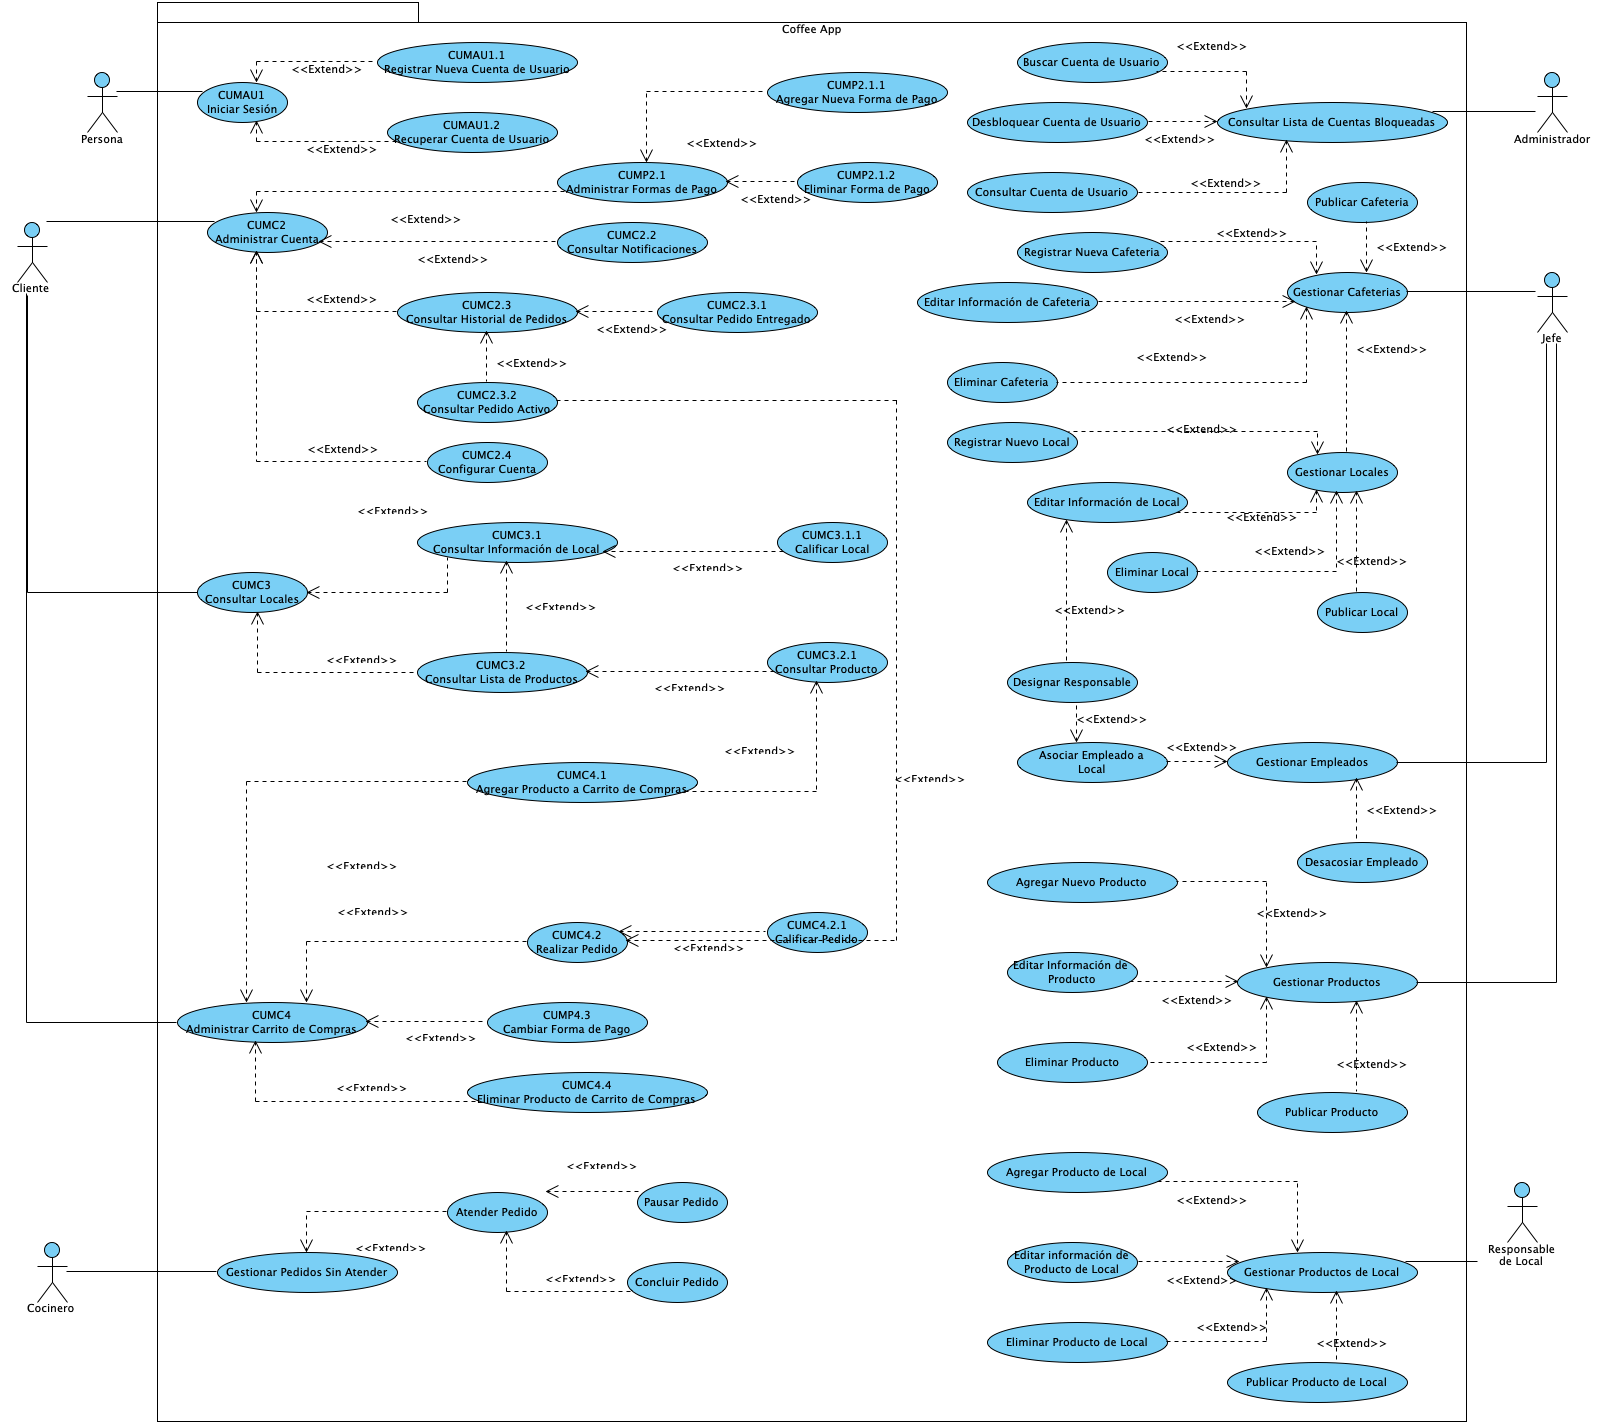
\includegraphics[angle=90,width=\textwidth]{img/cus}}
		\caption{Diagrama de Casos de Uso}
		\label{fig:casosDeUso}
	\end{center}
\end{figure}


\section{Interfaces de Usuario}
En la figura \ref{fig:mapaDeNavegacion} se utiliza una máquina de estados para presentar el camino ideal que se debe seguir para el uso de la aplicación móvil.

\begin{figure}[hbtp!]
	\begin{center}
		\fbox{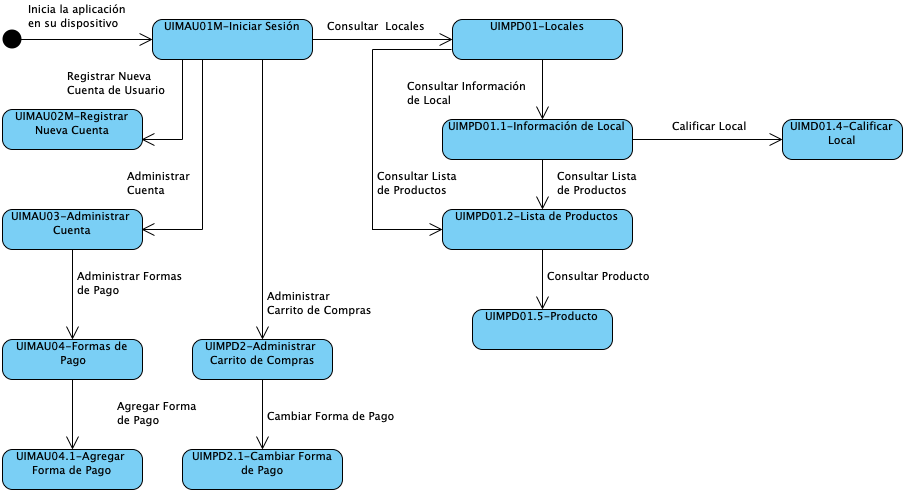
\includegraphics[width=0.8\textwidth]{img/mapaDeNavegacion}}
		\caption{Mapa de Navegación}
		\label{fig:mapaDeNavegacion}
	\end{center}
\end{figure}

%%!TEX root = ../../prueba.tex
\begin{IU}{IUMC3}{Consultar Locales}{En esta pantalla se muestran los locales que están cerca de la ubicación del \getElementById[Stakeholder]{Cliente}. Así mismo el cliente podrá realizar la búsqueda de un Local sí conociese su nombre o algunas palabras de su nombre. La pantalla desplegará la siguiente información del local:	\begin{Citemize}
		\item \getElementById[Entidad]{local.foto}.
		\item \getElementById[Entidad]{local.nombreLocal}.
		\item \getElementById[Entidad]{local.horaInicio}.
		\item \getElementById[Entidad]{local.horaFin}.
	\end{Citemize}}{casosDeUso/cumc3/IUMC3}
	\item[Acciones]:\hspace{1pt}
		\begin{Citemize}
			\item Al seleccionar un local se mostrarán los productos que se ofertan en ese local tal como se describe en el caso de uso \getElementById[CU]{CUMC3.2}.
			\item Al ingresar texto \fbox{Buscar cafetería} se realizará la búsqueda de los locales que contengan parte del texto ingresado.
		\end{Citemize}

\end{IU}



	
	\newpage
	\clossing
	
	%\saveData
\end{document}
